\clearpage
\subsubsection{Enumeration} % (fold)
\label{ssub:enum}

An Enumeration allows you to create a type where the value is one of a list of available options. When you declare an enumeration you are listing the values that are available for data of this type. The example in \fref{fig:type-decl-enum} declares a type that can have the value \texttt{ADD\_COINS} or \texttt{REMOVE\_COINS}.

\begin{figure}[h]
   \centering
   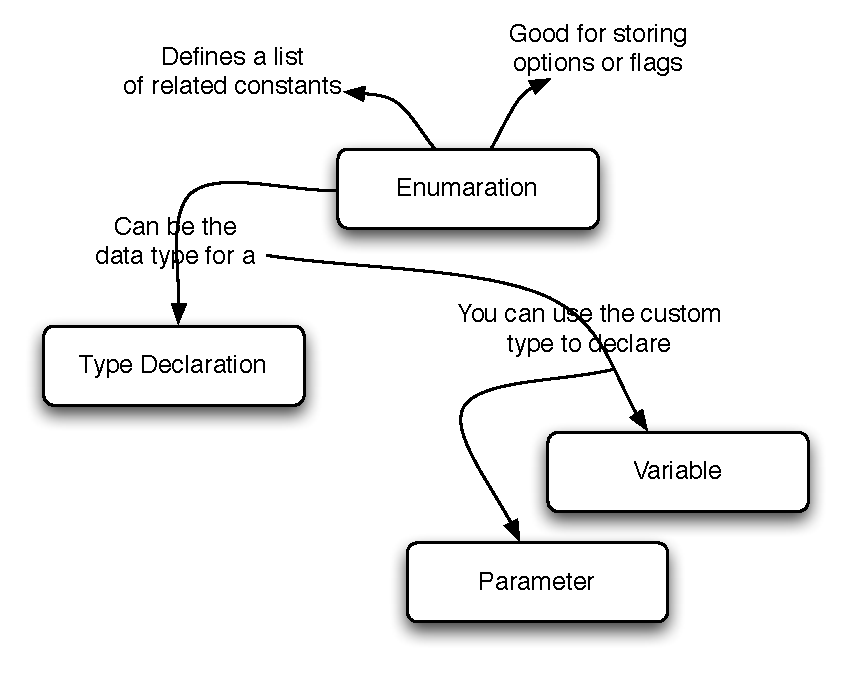
\includegraphics[width=\textwidth]{./topics/type-decl/diagrams/Enum} 
   \caption{An Enumeration allows you to define related constants}
   \label{fig:type-decl-enum}
\end{figure}

\mynote{
\begin{itemize}
  \item An Enumeration is a kind of \textbf{artefact} that you can declare.
  \item Using an enumeration you can declare a kind of value that must come from a list of available options.
  \item When you declare the enumeration you list the \emph{values} that it may have.
  \item This is like a list of constants, where values of this type will match one of these constants.
  \item Internally the compiler will map your values to numeric values. The first option is represented by the value \texttt{0}, the second is represented by the value \texttt{1}, and so on.
  \item You can specify the values for each option in the enumeration, this can be useful if you want to be able to combine options in a single value. In these cases you give each option a bit unique value (first at \texttt{1}, then \texttt{2}, \texttt{4}, \texttt{8}, \texttt{16}, etc).
  \item The \textbf{size} of an enumeration is based on the size of the integer type used to represent its values.
\end{itemize}
}

% subsection enumerations (end)